%iffalse
\let\negmedspace\undefined
\let\negthickspace\undefined
\documentclass{article}
\usepackage{cite}
\usepackage{amsmath,amssymb,amsfonts,amsthm}
\usepackage{algorithmic}
\usepackage{graphicx}
\usepackage{textcomp}
\usepackage{xcolor}
\usepackage{txfonts}
\usepackage{listings}
\usepackage{enumitem}
\usepackage{mathtools}
\usepackage{float}
\usepackage{gensymb}
\usepackage{comment}
\usepackage[breaklinks=true]{hyperref}
\usepackage{tkz-euclide} 
\usepackage{listings}
\usepackage{gvv}                                        
\def\inputGnumericTable{}                                 
\usepackage[latin1]{inputenc}                                
\usepackage{color}                                            
\usepackage{array}                                             
\usepackage{longtable}                                       
\usepackage{calc}                                             
\usepackage{multirow}                                         
\usepackage{hhline}                                           
\usepackage{ifthen}                                           
\usepackage{lscape}
\usepackage{multicol}

\newtheorem{theorem}{Theorem}[section]
\newtheorem{problem}{Problem}
\newtheorem{proposition}{Proposition}[section]
\newtheorem{lemma}{Lemma}[section]
\newtheorem{corollary}[theorem]{Corollary}
\newtheorem{example}{Example}[section]
\newtheorem{definition}[problem]{Definition}
\newcommand{\BEQA}{\begin{eqnarray}}
\newcommand{\EEQA}{\end{eqnarray}}
\newcommand{\define}{\stackrel{\triangle}{=}}
\theoremstyle{remark}
\newtheorem{rem}{Remark}
\begin{document}

\bibliographystyle{IEEEtran}
\vspace{3cm}

\title{Scientific Calculator Project Report}
\author{EE224BTECH11044 - Muthyala koushik% <-this % stops a space
}
\date{}
\maketitle
\bigskip



\renewcommand{\thefigure}{\theenumi}
\renewcommand{\thetable}{\theenumi}



\section{Introduction}
This project implements a scientific calculator using the Arduino Uno. It supports basic arithmetic, trigonometric (and inverse) functions, logarithmic/exponential operations, and complex expressions with proper operator precedence. A JHD162A LCD display shows the results, while push buttons serve as input. A recursive descent parser evaluates expressions accurately and efficiently.

\section{Aim}
\begin{itemize}[noitemsep]
    \item Design a calculator that performs:
    \begin{itemize}[noitemsep]
        \item Arithmetic: \texttt{+}, \texttt{-}, \texttt{*}, \texttt{/}, \texttt{\textasciicircum}
        \item Trigonometry: \texttt{sin}, \texttt{cos}, \texttt{tan} (in degrees)
        \item Inverse Trigonometry: \texttt{asin}, \texttt{acos}, \texttt{atan} (in degrees)
        \item Log/Exp: \texttt{ln}, \texttt{log}, \texttt{exp}
        \item Others: \texttt{sqrt}, \texttt{abs}, \texttt{\%}
    \end{itemize}
    \item Evaluate expressions using a recursive descent parser with proper precedence and parentheses.
    \item Provide real-time feedback via a JHD162A LCD display.
    \item Optimize resource use on the Arduino Uno.
\end{itemize}

\section{Components Required}
\begin{itemize}[noitemsep]
    \item Arduino Uno
    \item JHD162A LCD display
    \item 14 Push buttons:
    \begin{itemize}[noitemsep]
        \item 10 for digits (0--9)
        \item Clear (\texttt{C}) and Enter (\texttt{=})
        \item 2 Shift buttons: Arithmetic Shift (Shift-A) and Scientific Shift (Shift-S)
    \end{itemize}
    \item Wires, breadboard
\end{itemize}

\section{Hardware Configuration}
\subsection{Pin Connections}
\subsubsection{LCD Display (4-bit Mode)}
\begin{center}
\begin{tabular}{|l|l|l|}
\hline
\textbf{LCD Pin} & \textbf{Function} & \textbf{Arduino Pin} \\ \hline
RS             & Register Select & D8 (PB0) \\ \hline
E              & Enable          & D9 (PB1) \\ \hline
D4             & Data Bit 4      & D10 (PB2) \\ \hline
D5             & Data Bit 5      & D11 (PB3) \\ \hline
D6             & Data Bit 6      & D12 (PB4) \\ \hline
D7             & Data Bit 7      & D13 (PB5) \\ \hline
\end{tabular}
\end{center}
Additional connections: VSS (GND), VDD (+5V), VO (potentiometer), RW (GND), A (+5V backlight), K (GND).

\subsubsection{Push Button Connections}
\begin{center}
\begin{tabular}{|l|l|l|}
\hline
\textbf{Button}  & \textbf{Function}         & \textbf{Arduino Pin} \\ \hline
Digits 0--5    & Enter digits 0--5         & D2, D3, D4, D5, D6, D7 \\ \hline
Digits 6--9    & Enter digits 6--9         & A0, A1, A2, A3 \\ \hline
Clear (\texttt{C})    & Clear input                & A4 \\ \hline
Enter (\texttt{=})   & Evaluate expression        & A5 \\ \hline
Extra Button 1 & Additional function       & (Assign as needed) \\ \hline
Extra Button 2 & Additional function       & (Assign as needed) \\ \hline
\end{tabular}
\end{center}

\subsubsection{Shift Button Connections}
\begin{center}
\begin{tabular}{|l|l|l|}
\hline
\textbf{Button}               & \textbf{Function}          & \textbf{Arduino Pin} \\ \hline
Arithmetic Shift (Shift-A)    & Toggle arithmetic mode   & D0 (PD0) \\ \hline
Scientific Shift (Shift-S)    & Toggle scientific mode     & D1 (PD1) \\ \hline
\end{tabular}
\end{center}

\subsubsection{Power Supply}
\begin{center}
\begin{tabular}{|l|l|}
\hline
\textbf{Supply} & \textbf{Connection} \\ \hline
VCC           & +5V \\ \hline
GND           & Ground \\ \hline
\end{tabular}
\end{center}

\newpage

\begin{figure}[h!]
    \centering
    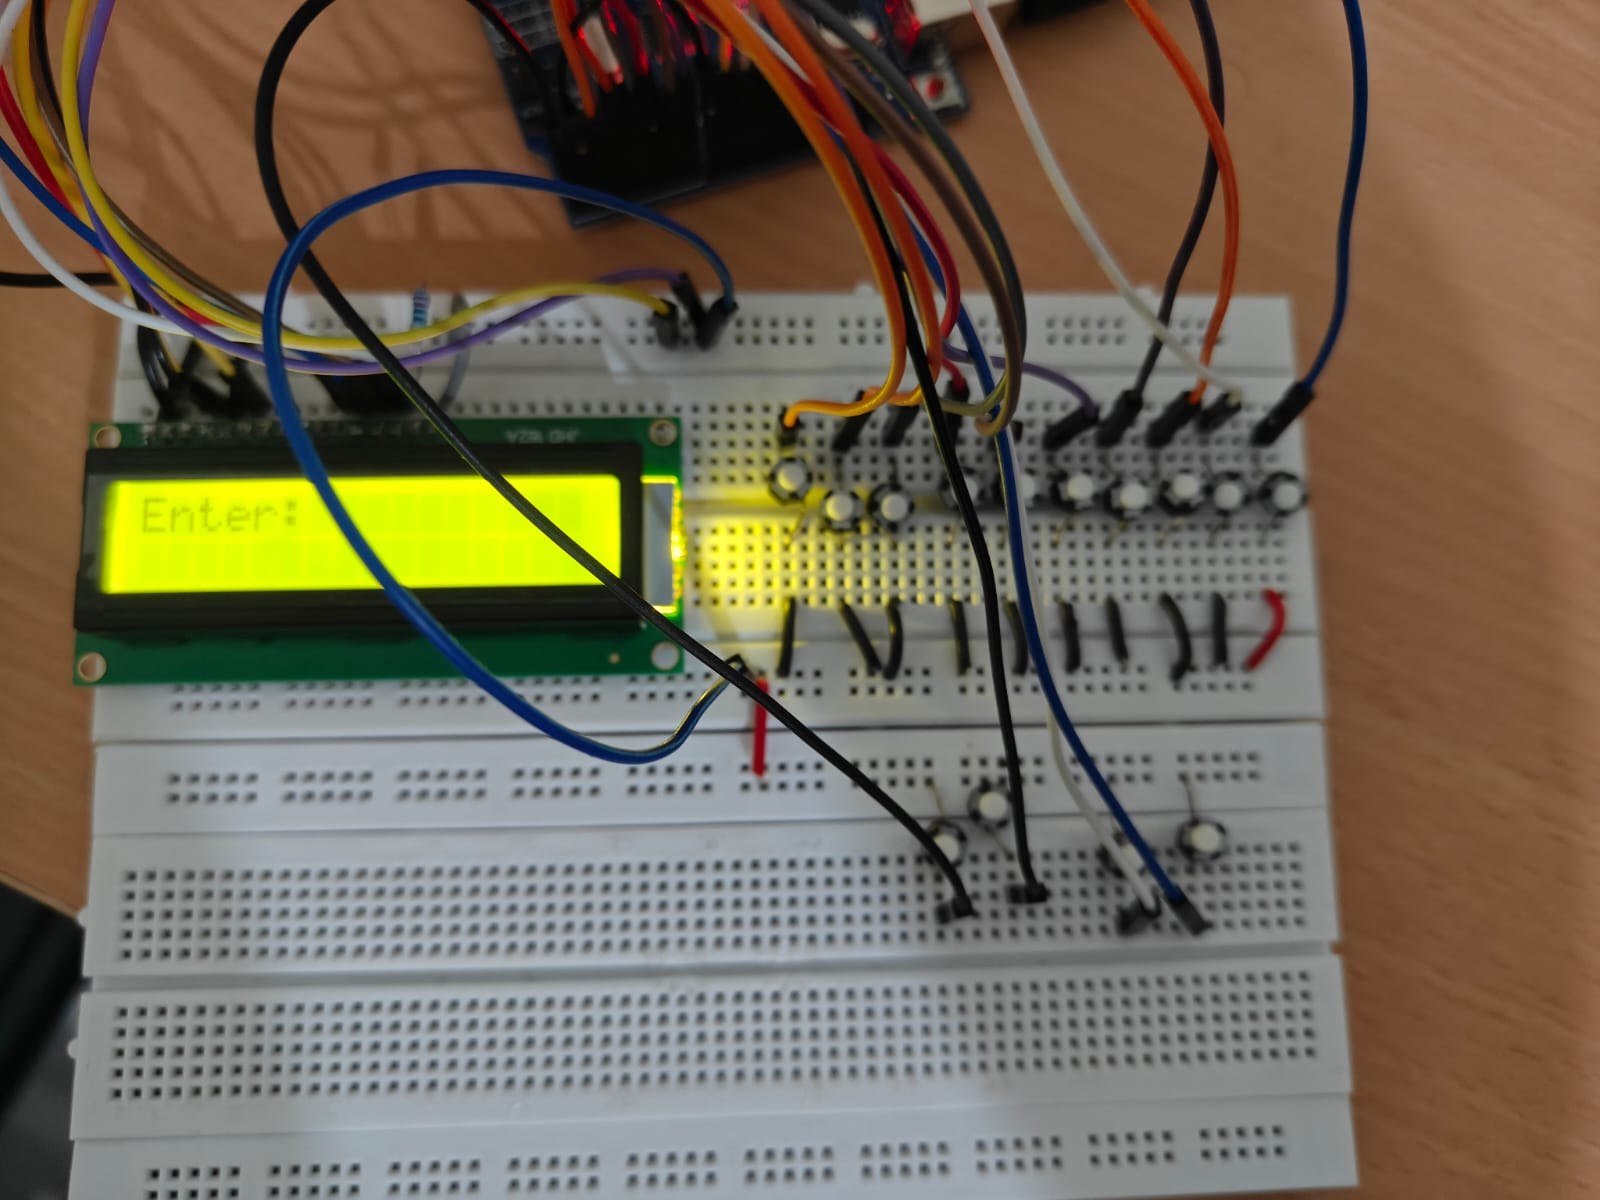
\includegraphics[width=0.9\columnwidth]{figs/circuit.png}
    \caption{Circuit diagram of the scientific calculator using Arduino Uno and JHD162A LCD}
    \label{fig:circuit_diagram}
\end{figure}


\section{Software Design}
\subsection{Overall Architecture}
The software is modular, divided into:
\begin{enumerate}[label=\alph*)]
    \item \textbf{Input Handling}: Scans push buttons, applies a 30 ms debounce delay, and detects mode switches.
    \item \textbf{User Interface (UI)}: Updates the LCD with the current expression, mode menus, and results. It initializes the LCD (4-bit mode), clears the screen, and sets the cursor.
    \item \textbf{Expression Evaluation}: Implements a recursive descent parser that enforces operator precedence, handles parentheses, and supports function calls.
\end{enumerate}

\subsection{Input Handling}
\begin{itemize}[noitemsep]
    \item \textbf{Button Scanning}: Uses \texttt{digitalRead()} to poll each push button.
    \item \textbf{Debouncing}: A 30 ms delay is applied to prevent false triggers.
    \item \textbf{Mode Switching}: Shift-A and Shift-S buttons toggle between arithmetic and scientific modes.
\end{itemize}

\subsection{User Interface (UI)}
\begin{itemize}[noitemsep]
    \item \textbf{LCD Initialization}: Functions like \texttt{lcd\_init()}, \texttt{lcd\_clear()}, and \texttt{lcd\_setCursor()} prepare the display.
    \item \textbf{Dynamic Display}: The current expression and mode menus are shown in real time. Error messages and results (to 4 decimal places) are displayed as needed.
\end{itemize}

\subsection{Expression Evaluation (Recursive Descent Parser)}
\begin{itemize}[noitemsep]
    \item \textbf{Operator Precedence}: 
    \begin{enumerate}[noitemsep]
        \item Level 1: \texttt{+} and \texttt{-}
        \item Level 2: \texttt{*}, \texttt{/}, and \texttt{\%}
        \item Level 3: \texttt{\textasciicircum} (right-associative)
    \end{enumerate}
    \item \textbf{Parentheses}: Extraneous outer parentheses are removed.
    \item \textbf{Function Support}: Recognizes and evaluates:
    \begin{itemize}[noitemsep]
        \item Trigonometric: \texttt{sin}, \texttt{cos}, \texttt{tan} (in degrees)
        \item Inverse Trigonometric: \texttt{asin}, \texttt{acos}, \texttt{atan} (in degrees)
        \item Log/Exp: \texttt{exp}, \texttt{ln}, \texttt{log}
        \item Others: \texttt{sqrt}, \texttt{abs}
    \end{itemize}
    \item \textbf{Numerical Methods}: Utilizes Euler's method, Newton-Raphson, and Riemann sums for approximations.
\end{itemize}

\subsection{Shift Modes}
\begin{itemize}[noitemsep]
    \item \textbf{Arithmetic Shift Mode (Shift-A)}:
    \begin{itemize}[noitemsep]
        \item \textbf{Navigation}: Use buttons 8 (Next) and 9 (Prev) to switch pages.
        \item \textbf{Mapping}: 
        \begin{itemize}[noitemsep]
            \item Page 0: \texttt{+}, \texttt{-}, \texttt{*}, \texttt{/}
            \item Page 1: \texttt{\textasciicircum}, \texttt{\%}, \texttt{(}, \texttt{)}
            \item Page 2: Backspace (BS)
        \end{itemize}
    \end{itemize}
    \item \textbf{Scientific Shift Mode (Shift-S)}:
    \begin{itemize}[noitemsep]
        \item \textbf{Navigation}: Use buttons 8 and 9 for page control.
        \item \textbf{Mapping}: 
        \begin{itemize}[noitemsep]
            \item Page 0: \texttt{sin}, \texttt{cos}, \texttt{tan}, \texttt{exp}
            \item Page 1: \texttt{ln}, \texttt{sqrt}, \texttt{log}, \texttt{abs}
            \item Page 2: \texttt{asin}, \texttt{acos}, \texttt{atan}
        \end{itemize}
    \end{itemize}
\end{itemize}
The LCD displays the current mode and page for user guidance.

\subsection{AVR GCC}
The firmware is compiled using AVR GCC, part of the AVR toolchain. AVR GCC enables code optimization for size and speed on resource-constrained systems like the Arduino Uno. It supports inline assembly for performance-critical sections and works in conjunction with avr-libc and avrdude for programming the microcontroller.

\subsection{Error Handling}
\begin{itemize}[noitemsep]
    \item Checks for division by zero, mismatched parentheses, and domain errors (e.g., \texttt{sqrt} of a negative number).
    \item Invalid selections in shift modes trigger brief error messages.
\end{itemize}

\section{Operation Workflow}
\begin{enumerate}
    \item \textbf{Startup}: The LCD shows "Simple Calc" for 2 seconds, then displays "Enter:".
    \item \textbf{Normal Mode}: Users input digits and operators; pressing \texttt{=} evaluates the expression.
    \item \textbf{Shift Modes}: Toggled by Shift-A (D0) or Shift-S (D1); navigation with buttons 8/9; selection with buttons 0--3.
    \item \textbf{Result}: Displayed to 4 decimal places; new input clears the result.
\end{enumerate}

\section{Performance Specifications}
\begin{itemize}[noitemsep]
    \item \textbf{Voltage}: 5V DC
    \item \textbf{Current}: $\sim$50 mA (active), $<$10 mA (idle)
    \item \textbf{Precision}: IEEE 754 emulation; results to 4 decimal places.
    \item \textbf{Expression Limit}: 64 characters.
    \item \textbf{Speed}: Arithmetic $<$10 ms; trigonometric $\sim$200 ms.
\end{itemize}

\section{AVR Code Explanation}

The embedded C code for the Arduino Uno is structured modularly to manage LCD interfacing, button inputs, expression parsing, and evaluation. The key components of the code are described below.

\subsection{1. LCD Initialization and Display}

The LCD used is a JHD162A, interfaced in 4-bit mode using Arduino Uno's digital pins D8--D13. Initialization is done using \texttt{lcd\_init()}, which sends the necessary commands for enabling display, clearing the screen, and setting cursor behavior.

\begin{itemize}
    \item \texttt{lcd\_cmd(uint8\_t cmd)}: Sends control commands (e.g., clear, home).
    \item \texttt{lcd\_data(char ch)}: Sends a character to be printed on screen.
    \item \texttt{lcd\_print(char *s)}: Prints a full string on the LCD.
\end{itemize}

\subsection{2. Button Scanning and Input}

Buttons are connected to D2--D7 and A0--A5, and are scanned using the \texttt{read\_buttons()} function. The button press is debounced and mapped to a character or command such as digit, operator, clear, or shift.

\begin{itemize}
    \item Inputs are buffered into a character array \texttt{expr[64]} as the user types.
    \item Each character is appended until `=' is pressed to trigger evaluation.
\end{itemize}

\subsection{3. Expression Parsing and Evaluation}

A recursive descent parser is implemented to handle operator precedence, parentheses, and scientific functions. The input is parsed using the following hierarchy:

\begin{itemize}
    \item \texttt{parse\_expression()}: Handles `+' and `-'
    \item \texttt{parse\_term()}: Handles `*', `/', and modulus
    \item \texttt{parse\_factor()}: Handles numbers, parentheses, and powers
    \item \texttt{parse\_function()}: Handles function names like \texttt{sin}, \texttt{log}, \texttt{sqrt}, etc.
\end{itemize}

The result is computed and returned to be displayed on the LCD.

\subsection{4. Scientific Functions (Manual Implementation)}

Common scientific functions are implemented manually using numerical approximations:

\begin{itemize}
    \item \texttt{sin\_deg(double x)}: Computes $\sin(x)$ using Taylor series in degrees.
    \item \texttt{log\_custom(double x)}: Approximates $\log_{10}(x)$ using iterative or series methods.
    \item \texttt{sqrt\_custom(double x)}: Uses Newton-Raphson method for square roots.
\end{itemize}

This approach avoids using standard math libraries, reducing code size and allowing better control on AVR.

\subsection{5. Shift Modes for Multi-Function Input}

To maximize button usage, shift modes are introduced:

\begin{itemize}
    \item \texttt{Shift-A (Arithmetic)} and \texttt{Shift-S (Scientific)} buttons change input context.
    \item With 2 shift modes and multiple pages, a small number of buttons can cover all necessary operations.
    \item The mapping is handled using flags and arrays that define the current page and mode.
\end{itemize}

\subsection{6. Display and Error Handling}

The calculator continuously updates the display with current input. Upon pressing `=', the expression is evaluated and the result is shown with 4-digit precision.

\begin{itemize}
    \item Errors like division by zero, invalid syntax, or domain errors (e.g., $\sqrt{-1}$) are detected and a message like \texttt{Error} is displayed temporarily.
\end{itemize}

\subsection{7. Main Loop}

The \texttt{main()} function initializes the LCD and runs an infinite loop to manage input and output.

\begin{verbatim}
int main() {
    lcd_init();
    show_welcome();
    while (1) {
        handle_input();
        update_lcd();
    }
}
\end{verbatim}

\begin{itemize}
    \item \texttt{handle\_input()}: Reads buttons and updates the expression.
    \item \texttt{update\_lcd()}: Refreshes the display based on the current state.
\end{itemize}
\end{document}
